\subsection{Увеличение резкости}

Для увеличения резкости воспользуемся матрицей

\begin{gather}
    K = \begin{pmatrix}
        0 & -1 & 0\\
        -1 & 5 & 1-\\
        0 & -1 & 0
    \end{pmatrix}  
\end{gather}

Получим результат применения этой матрицы на изображение посредством свёртки и Фурье-преобразований:

\begin{figure}[ht!]
    \centering
    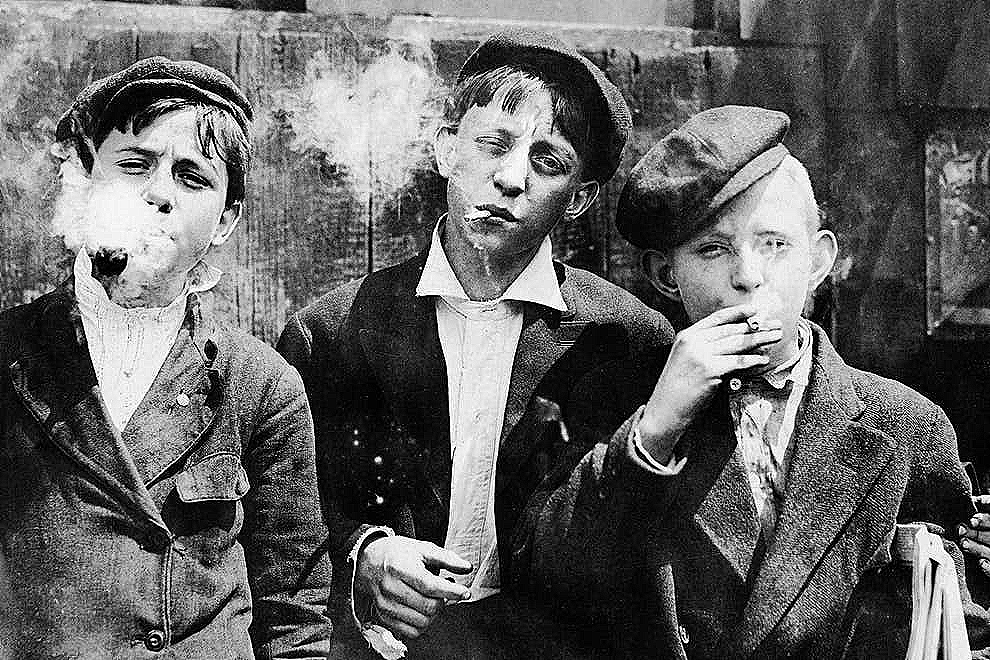
\includegraphics[width=0.95\textwidth]{images/result/task_3/Sharpened.png}
    \caption{Увеличение резкости изображения при помощи свертки}
    \label{fig:sh_c_5}
\end{figure}

\begin{figure}[ht!]
    \centering
    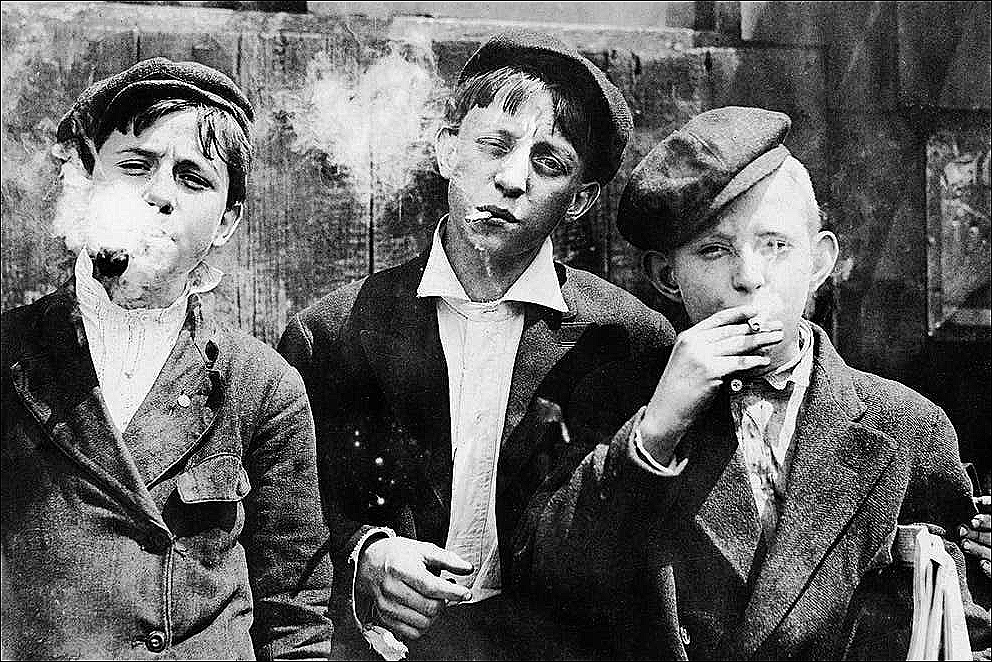
\includegraphics[width=0.95\textwidth]{images/result/task_3/Sharpened_fourier.png}
    \caption{Увеличение резкости изображения при помощи преобразований Фурье}
    \label{fig:sh_f_5}
\end{figure}
\clearpage
Полученные изображения идентичны друг другу. Единственное различие -- на изображении, полученном при использовании свертки, отсутствуют темные границы, так как свертка реализована при помощи функции \textit{filter2D()} из библиотеки \textit{OpenCV-Python}.